\documentclass[[12pt,DIV14,BCOR12mm,a4paper,footexclude,headinclude,halfparskip-,twoside,openright,cleardoubleempty,idxtotoc,bibtotoc]{article}

\usepackage[textwidth=16cm,textheight=26cm]{geometry}
%\usepackage[top=3cm,bottom=2]{geometry}


\usepackage{graphicx}
\usepackage[english]{babel}
%\usepackage[font={small}]{caption}
\usepackage[font=small,format=hang]{subcaption}
\usepackage[font=small,format=hang]{caption}
%\usepackage[format=hang]{caption}       % for hanging captions
%\usepackage{subfig}                     % for subfigures
\usepackage{wrapfig}                    % for figures floating in text, alternatively you can use >>floatflt<<
\usepackage{pifont}

\usepackage{tikz}
\usetikzlibrary{arrows,positioning,shapes.geometric, calc, shadows, decorations.pathreplacing, patterns, hobby}


\usepackage{hyperref}


%\usepackage[table]{xcolor}

%%%%%%%%%%%%%%%%%%%%%%%%%%%%%%%




\begin{document}

\title{The Livius Documentation}
\author{Author: Parnia Bahar}

\maketitle

\begin{abstract}
This Documentation serves as a short description for all required knowledge and previous works regarding the LiVius project in Max-Planck institute of intelligent system, Empirical Inference department. The main aim of the work is to automatically create an appropriate layout for online courses and lectures.  In this case, a proper framework should be composed of both the lecture slides and the speaker/teacher. To this aim, computer vision and machine learning  based algorithms are applied.
\end{abstract}

\section{Introduction}

There are many advantages to online and computer-based learning when compared to traditional face-to-face courses and lectures, however, there are a few disadvantages as well.
Online courses are great for self-motivated individuals who want to learn new skills and advance their careers and their knowledge without attending in the college or university. Getting education online will also save tons of money. Although some would argue that online education is only an awesome alternative to traditional education because of the savings and convenience, there are actually many other advantages. Only online education fully integrates itself into today’s educational technology. It is also more efficient for fast and especially motivated learners and offers skills that lack resources in traditional education despite high demand from employers. 

Class work can be scheduled around work and family.
Reduces travel time and travel costs for off-campus students.
Students may have the option to select learning materials that meets their level of knowledge and interest.
Students can study anywhere they have access to a computer and Internet connection.
Self-paced learning modules allow students to work at their own pace.
Flexibility to join discussions in the bulletin board threaded discussion areas at any hour, or visit with classmates and instructors remotely in chat rooms.
Instructors and students both report e-Learning fosters more interaction among students and instructors than in large lecture courses.
e-Learning can accommodate different learning styles and facilitate learning through a variety of activities. Develops knowledge of the Internet and computers skills that will help learners throughout their lives and careers.
Successfully completing online or computer-based courses builds self-knowledge and self-confidence and encourages students to take responsibility for their learning.
Learners can test out of or skim over materials already mastered and concentrate efforts in mastering areas containing new. information and/or skills \cite{onlinecourse}.
Therefore, the demand of taking online classes is increasing and there are many universities and educational organizations which offer free online courses. 



\subsection{The Framework }
One can make see the whole framework of the project in the figure \ref{fig_framework}. The whole project can be divided into three major tasks. The first one is video processing and it is related to all algorithms and pre-processing steps for slide detection and speaker tracking. Here, the processing tasks can be done either on the video file itself or on the separate frames. The second one can be called video editing and it includes all necessary works for the codecs of the audio and video, the final layout, the background image, the logo and concatenating all together to form the final version of the  video. The third task is the streaming the prepared video on the Internet.


\subsection{Output video layout}

In order to broadcast the final video, the full HD size is used. The final video size to stream is 1920x1320. Figure \ref{fig_layout} depicts the final layout and the the title and background images.






\begin{figure}[ht]
\resizebox{1\linewidth}{!}{
\pgfdeclarelayer{background}
\pgfdeclarelayer{foreground}
\pgfsetlayers{background,main,foreground}

\begin{tikzpicture}[>=latex']

\tikzset{block/.style={
      rectangle,
      draw=blue,
      thick,
      fill=gray!20,
      text width=2.1cm,
      align=center,
      rounded corners,
      minimum height=2em
    },
    oblock/.style={
          rectangle,
          draw=blue,
          thick,
          fill=gray!20,
          text width=2.7cm,
          align=center,
          rounded corners,
          minimum height=2em
        }, 
rblock/.style={draw, shape=rectangle,rounded corners=1.5em,align=center,minimum height=4cm, text centered, text width= 3cm},
database/.style={draw, shape=cylinder, cylinder uses custom fill,
      shape border rotate=90, aspect=0.25,text centered, text width= 2.5cm, minimum height=3cm, fill=gray!20,
      draw=blue},
ann/.style= {above, text width=10em, text centered},
}


\node[inner sep=0pt] (video)  at (0,0) 
    { \includegraphics[width=0.15\textwidth]{figures/video.png}};

\node [block, above right =1cm of video]  (vp1) {Pre-Processing};
\node [block, above right  = 0.3cm of vp1]  (vp2) {Slide Detection};
\node [block, below =1.5cm of vp2]  (vp3) {Speaker Tracking};
\node [block, right =3cm of vp1]  (vp4) {Post-Processing};
\node [block, right =1cm of vp4]  (ve5) {Layout Concatenating};
\node [block, right =0.5cm of ve5]  (ve6) {Transcoding/ Filtering};
\node[inner sep=0pt,  below right =1cm of ve6] (layout)  { \includegraphics[width=0.15\textwidth]{figures/layout.png}};

\node [block, below right=2.5cm of video]  (ap1) {Equalizer};
\node [block, right=1cm of ap1]  (ap2) {Improvement};
\node [block, right =1cm of ap2]  (ap3) {Transcoding/ Filtering};
\node [block, right =1cm of ap3]  (ap4) {Final Audio file};

\node [ann, below right=1cm of vp4]  (bk) {Background Image};
\node [ann, below =0.01cm of bk]  (info) {Talk/Speaker Info.};

\begin{pgfonlayer}{background}
        \path (vp1.west |- vp2.north)+(-0.3,0.3) node (a) {};
        \path (vp3.south -| vp4.east)+(0.3,-0.3) node (b) {};       
        \path[fill=blue!10,rounded corners, draw=black!50, dashed]
            (a) rectangle (b);           
        \path (vp2.north)+(0.0,+0.5) node (a) {Video Processing};            
 \end{pgfonlayer}


\begin{pgfonlayer}{background}
        \path (ve5.west |- ve5.north)+(-0.3,0.3) node (a) {};
        \path (ve6.south -| ve6.east)+(0.3,-0.3) node (b) {};       
        \path[fill=blue!10,rounded corners, draw=black!50, dashed]
            (a) rectangle (b);           
        \path (ve5.north east)+(0.0,+0.5) node (a) {Video Editing};            
 \end{pgfonlayer}


\begin{pgfonlayer}{background}
        \path (ap1.west |- ap1.north)+(-0.3,0.3) node (a) {};
        \path (ap4.south -| ap4.east)+(0.3,-0.3) node (b) {};       
        \path[fill=blue!10,rounded corners, draw=black!50, dashed]
            (a) rectangle (b);           
        \path (ap2.north east)+(0.0,+0.5) node (a) {Audio Processing};            
 \end{pgfonlayer}



 paths
\path[draw,->] 
          	(vp1) edge (vp2)
          	(vp1) edge (vp3)
	 	(vp3) edge (vp4)
	  	(vp2) edge (vp4)
		(vp4) edge (ve5)
		(ve5) edge (ve6)

	  	(ap1) edge (ap2)
		(ap2) edge (ap3)
		(ap3) edge (ap4)
;
               
\draw[-latex] +(1,1.5) node (a) {Video}(video.east) -- ++(0.5,0)  |-  (vp1.west) ;
\draw[-latex] +(1,-1.5) node (a2) {Audio}(video.east) -- ++(0.5,0) |-  (ap1.west);

\draw[-latex] (ve6.east) -- ++(0.5,0) |-  (layout.west);
\draw[-latex] (ap4.east) -- ++(0.95,0) |-  (layout.west);

\draw[-latex] (bk.west) -- ++ (-0.2,0.0) |-  (ve5.west);
\draw[-latex] (info.west) -- ++(-0.2,0.0) |-  (ve5.west);


\end{tikzpicture}
}
\vspace{-0.3cm}
    \caption{\small The whole framework}
    \label{fig_framework}
\centering
\end{figure}




\begin{figure}[ht]
	\centering

	\begin{subfigure}[b]{0.30\textwidth}
	\resizebox{1\linewidth}{!}{
\pgfdeclarelayer{background}
\pgfdeclarelayer{foreground}
\pgfsetlayers{background,main,foreground}

\begin{tikzpicture}[>=latex']

\draw (0,0)  node[xshift=-0.5cm,yshift= 2cm, text width=0.5cm, black ,font=\small]{1320} -- (6,0) -- (6,4) -- (0,4)  node[xshift=4.2cm,yshift= 0.2cm, text width=3cm, black ,font=\small]{1920} -- (0,0);
\draw[thick,-] (2,0) -- (2,4);
\draw[thick,-] (0,1.33)  -- (2,1.33) node[xshift=-1cm,yshift= 0.7cm, text width=1cm, black ,font=\small]{Speaker 640x360};
\draw[thick,-] (0,2.66) -- (2,2.66);
\draw[thick,-] (2,0.5) -- (6,0.5)  node[xshift=-2cm,yshift= 1.5cm, text width=1cm, black ,font=\small]{Slide 1280x960};
\draw[thick,-] (2,3.5) -- (6,3.5);

\end{tikzpicture}
}
	      \caption{\small Video layout}
		\label{fig_layout_a}
	\end{subfigure} 
	\begin{subfigure}[b]{0.30\textwidth}
	      \includegraphics[width=\textwidth]{figures/background_example.png}
	      \caption{\small Background image}
		\label{fig_layout_b}
	\end{subfigure}	       
	\begin{subfigure}[b]{0.30\textwidth}
	       \includegraphics[width=\textwidth]{figures/title_example.png}
	       \caption{\small First Info. slide}
	\label{fig_layout_c}
	\end{subfigure}
	\caption{The final video layout}
	\label{fig_layout}
\end{figure}







\section{Requirements}




\subsection{Hardware}

The current hardware and tools are shown in figure \ref{fig_hw}. Figure \ref{fig_hw_c} indicates the 4k Blackmagic Camera, its power supply, audio cables and the ultrasonic 24mm lens. Figure \ref{fig_hw_c} is the 2-TB USB3.0 external hard disk for any mobility.  Figure \ref{fig_hw_d} shows the 1-TB Solid State Drive (SSD) which suits with Blackmagic camera and \ref{fig_hw_d} includes Sata HDD docking station and reader along with its secondary power supply and USB3.0 port. Besides the shown laptop, there is another desktop PC as an implementation platform with following properties.

\begin{itemize}
	\item Processor: Intel® Core™ i7-5930K CPU @ 3.50GHz × 12 
	\item Memory: 32 GiB
	\item Graphic: NVIDIA GeForce GTX 750/PCIe/SSE2
	\item Disk: 3 Data raid for 12 TB
	\item Operating system: Ubuntu 14.04 and windows 7
\end{itemize}


\begin{figure}[ht]
	\centering
	\begin{subfigure}[b]{0.18\textwidth}
	       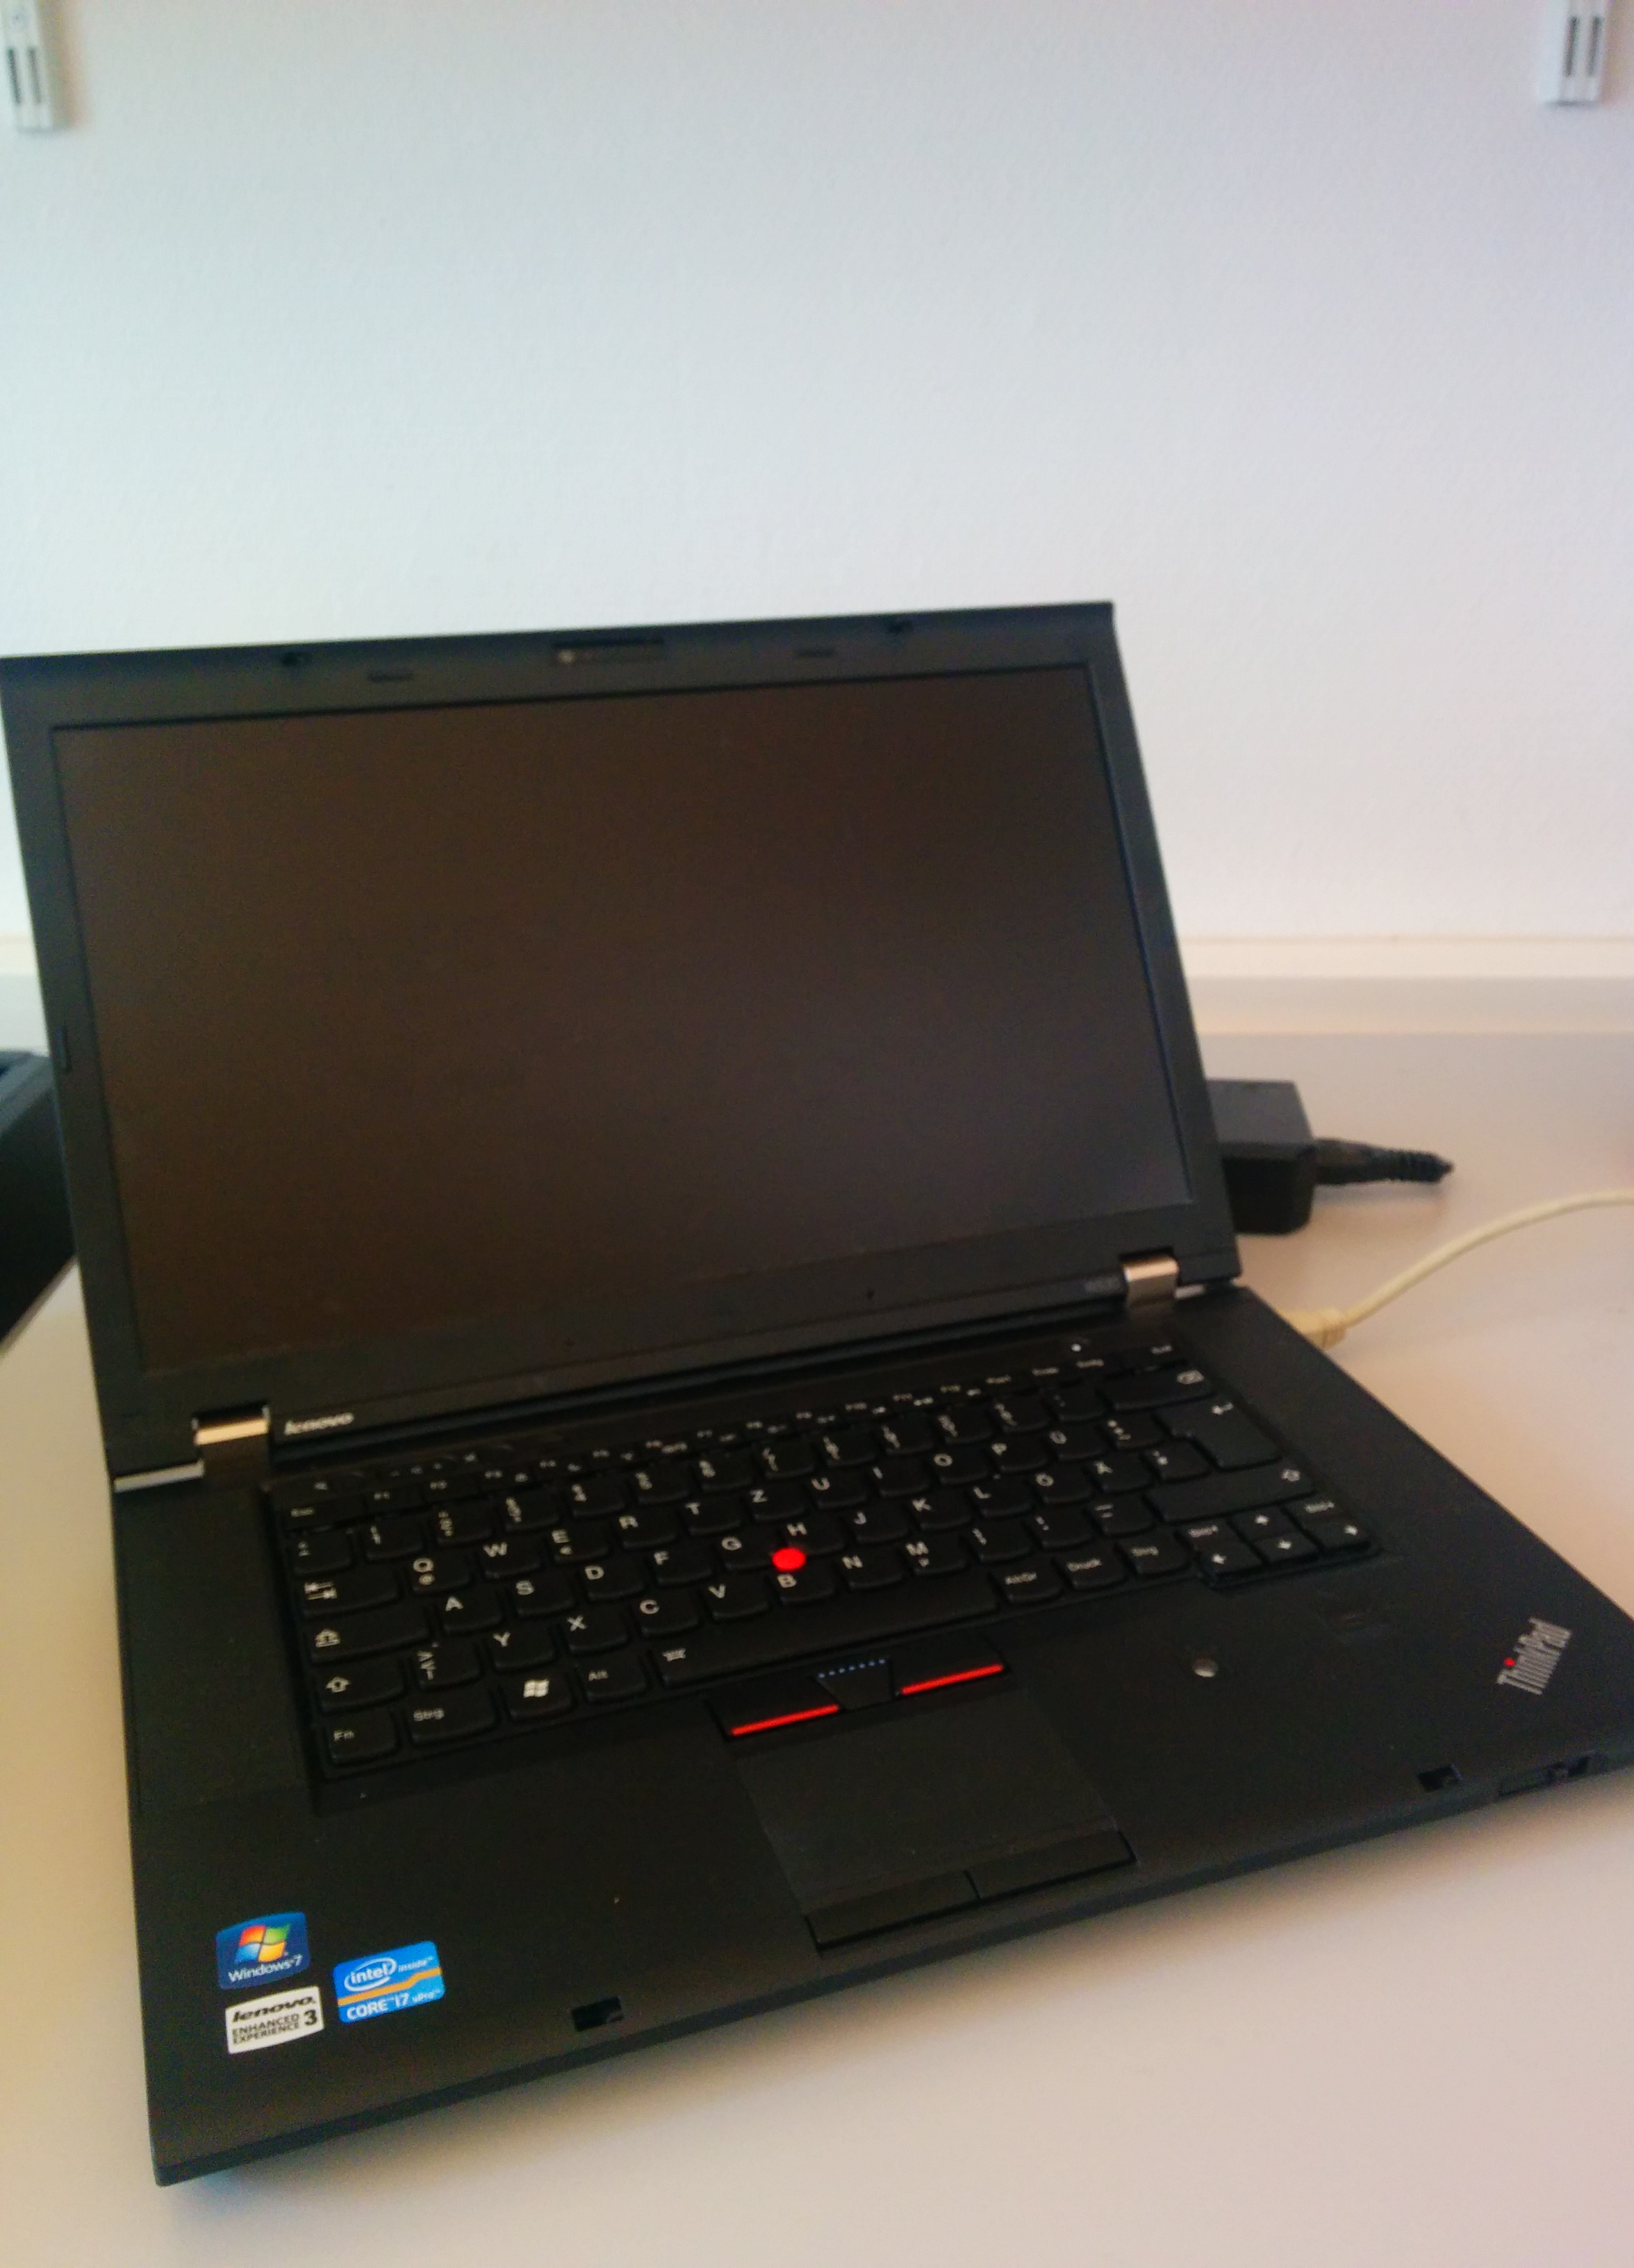
\includegraphics[width=\textwidth]{figures/1_(1).png}
	       \caption{}
		\label{fig_hw_a}
	\end{subfigure} 
	\begin{subfigure}[b]{0.18\textwidth}
	      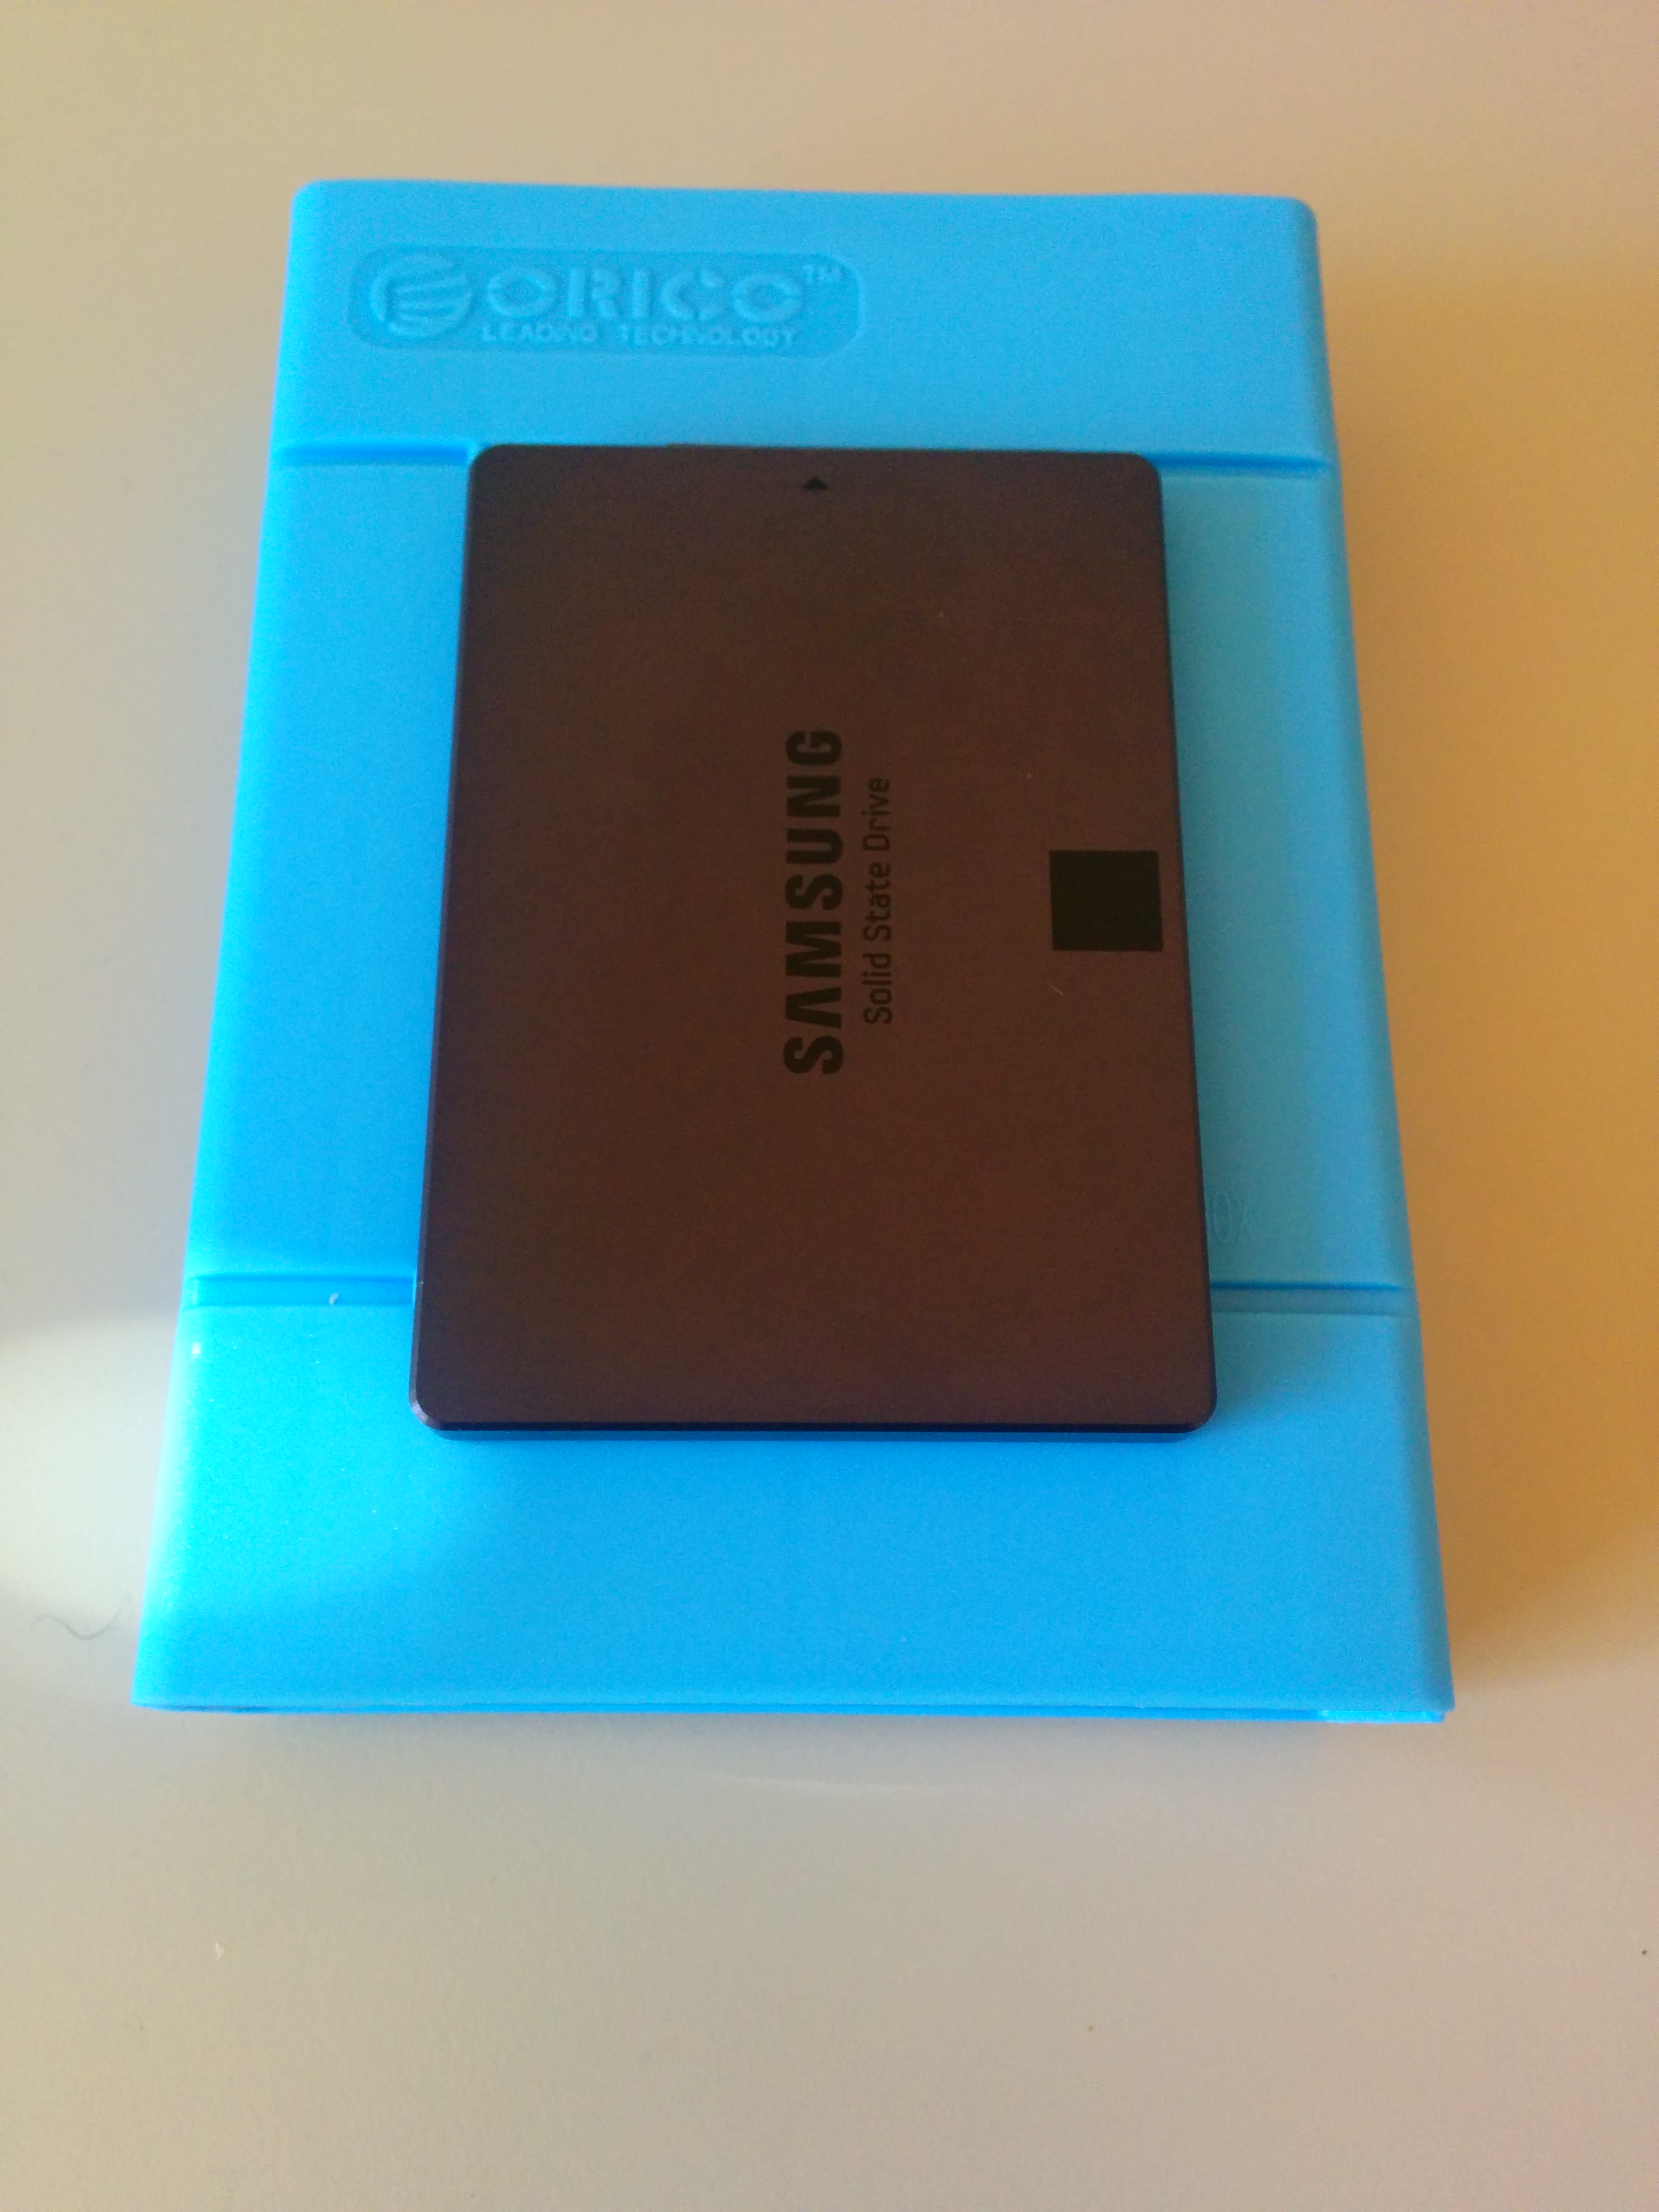
\includegraphics[width=\textwidth]{figures/1_(2).jpg}
	      \caption{}
		\label{fig_hw_b}
	\end{subfigure}	        
	\begin{subfigure}[b]{0.18\textwidth}
	       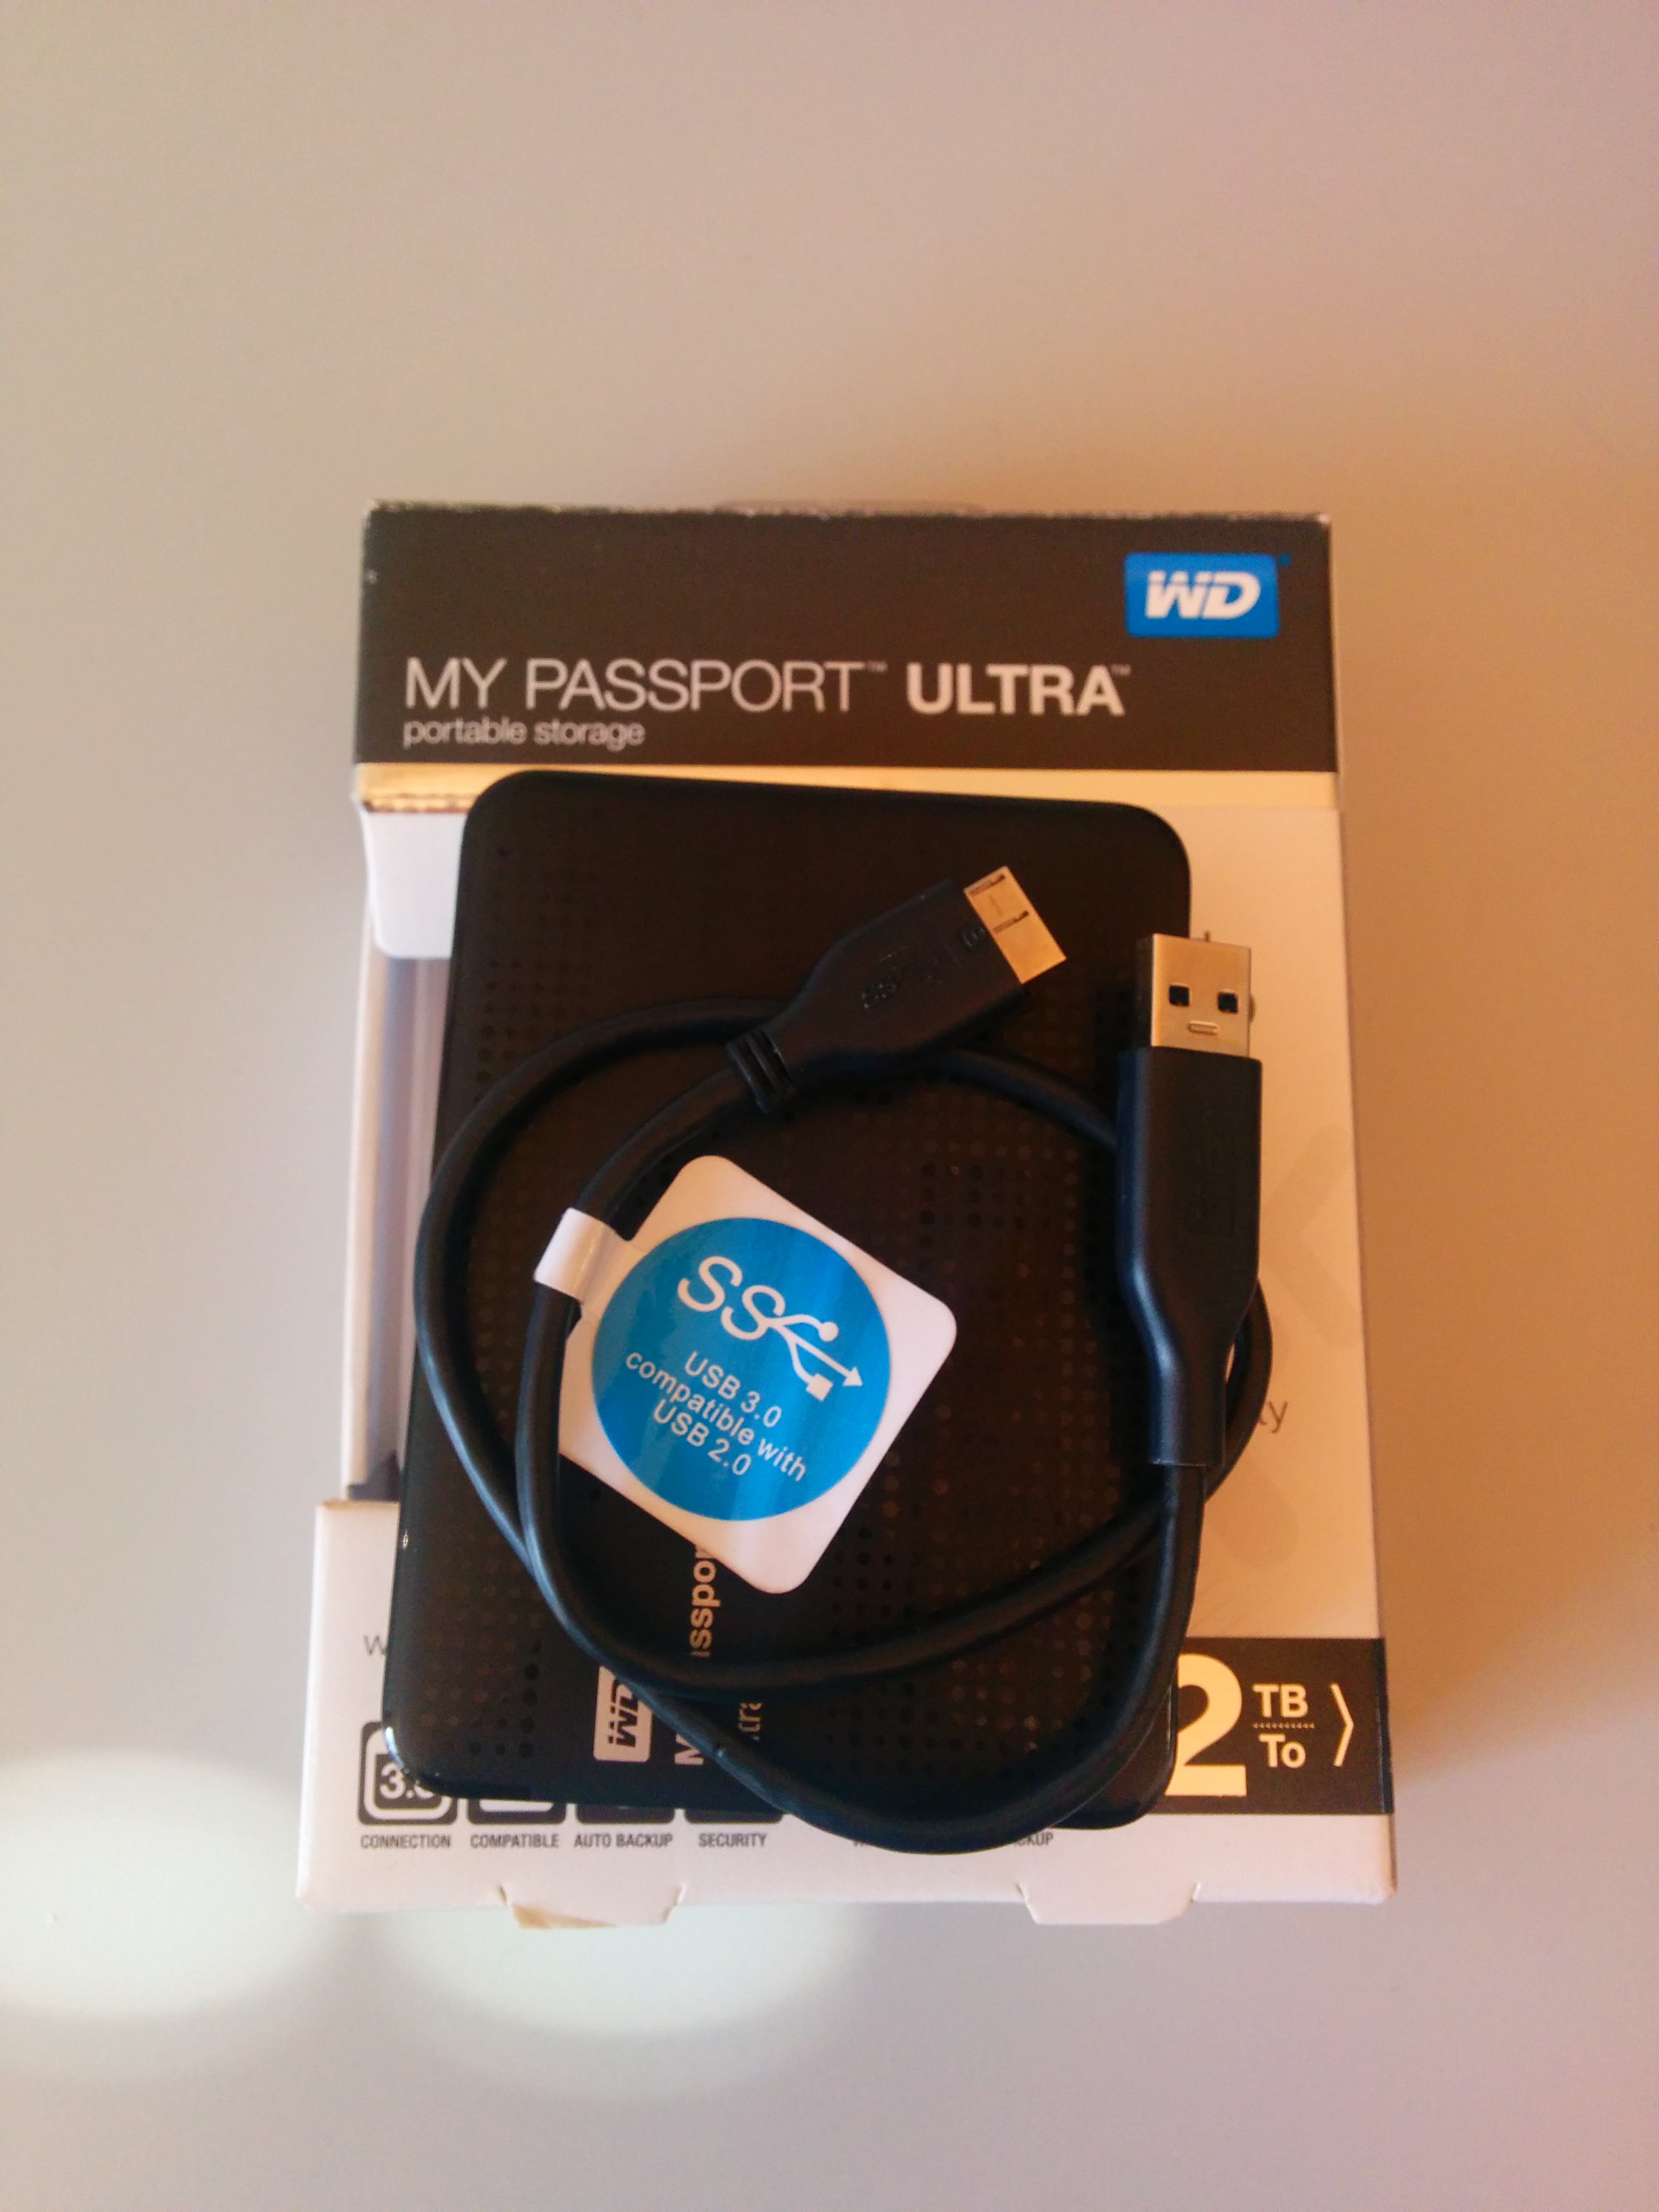
\includegraphics[width=\textwidth]{figures/1_(3).png}
	       \caption{}
	\label{fig_hw_c}
	\end{subfigure}
	\begin{subfigure}[b]{0.18\textwidth}
	      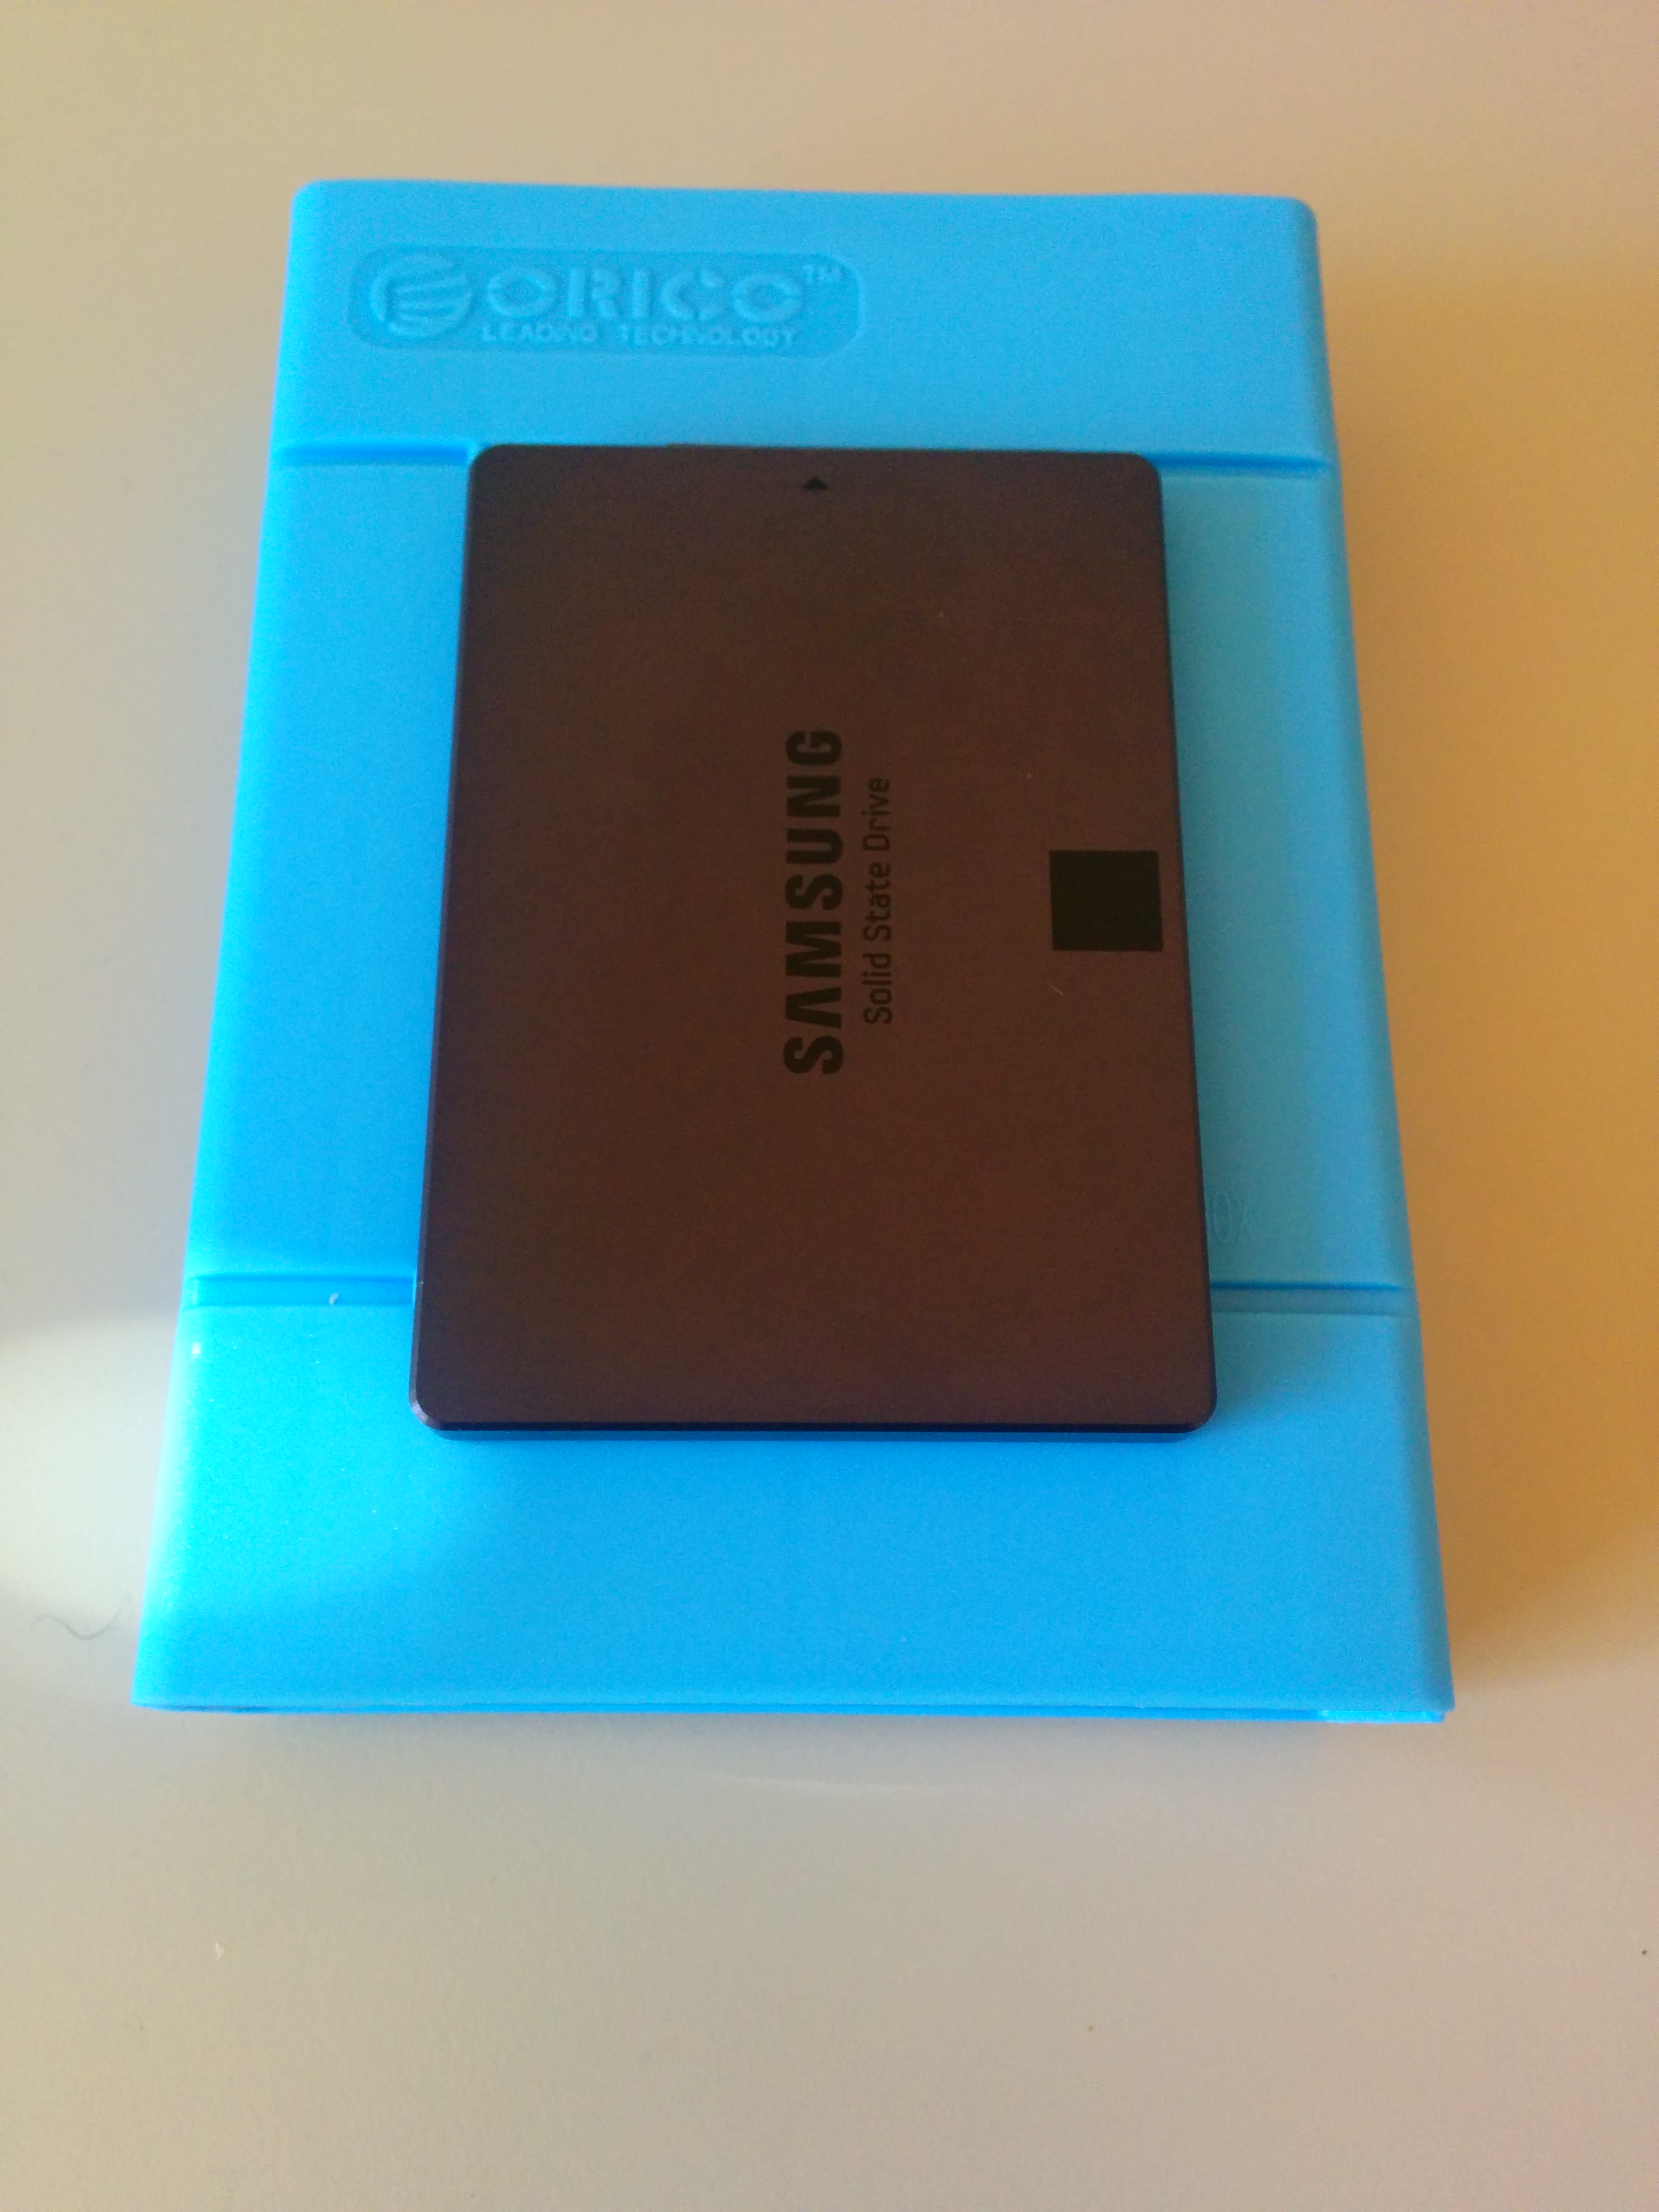
\includegraphics[width=\textwidth]{figures/1_(2).png}
	      \caption{}
		\label{fig_hw_d}
	\end{subfigure}
	\begin{subfigure}[b]{0.18\textwidth}
	      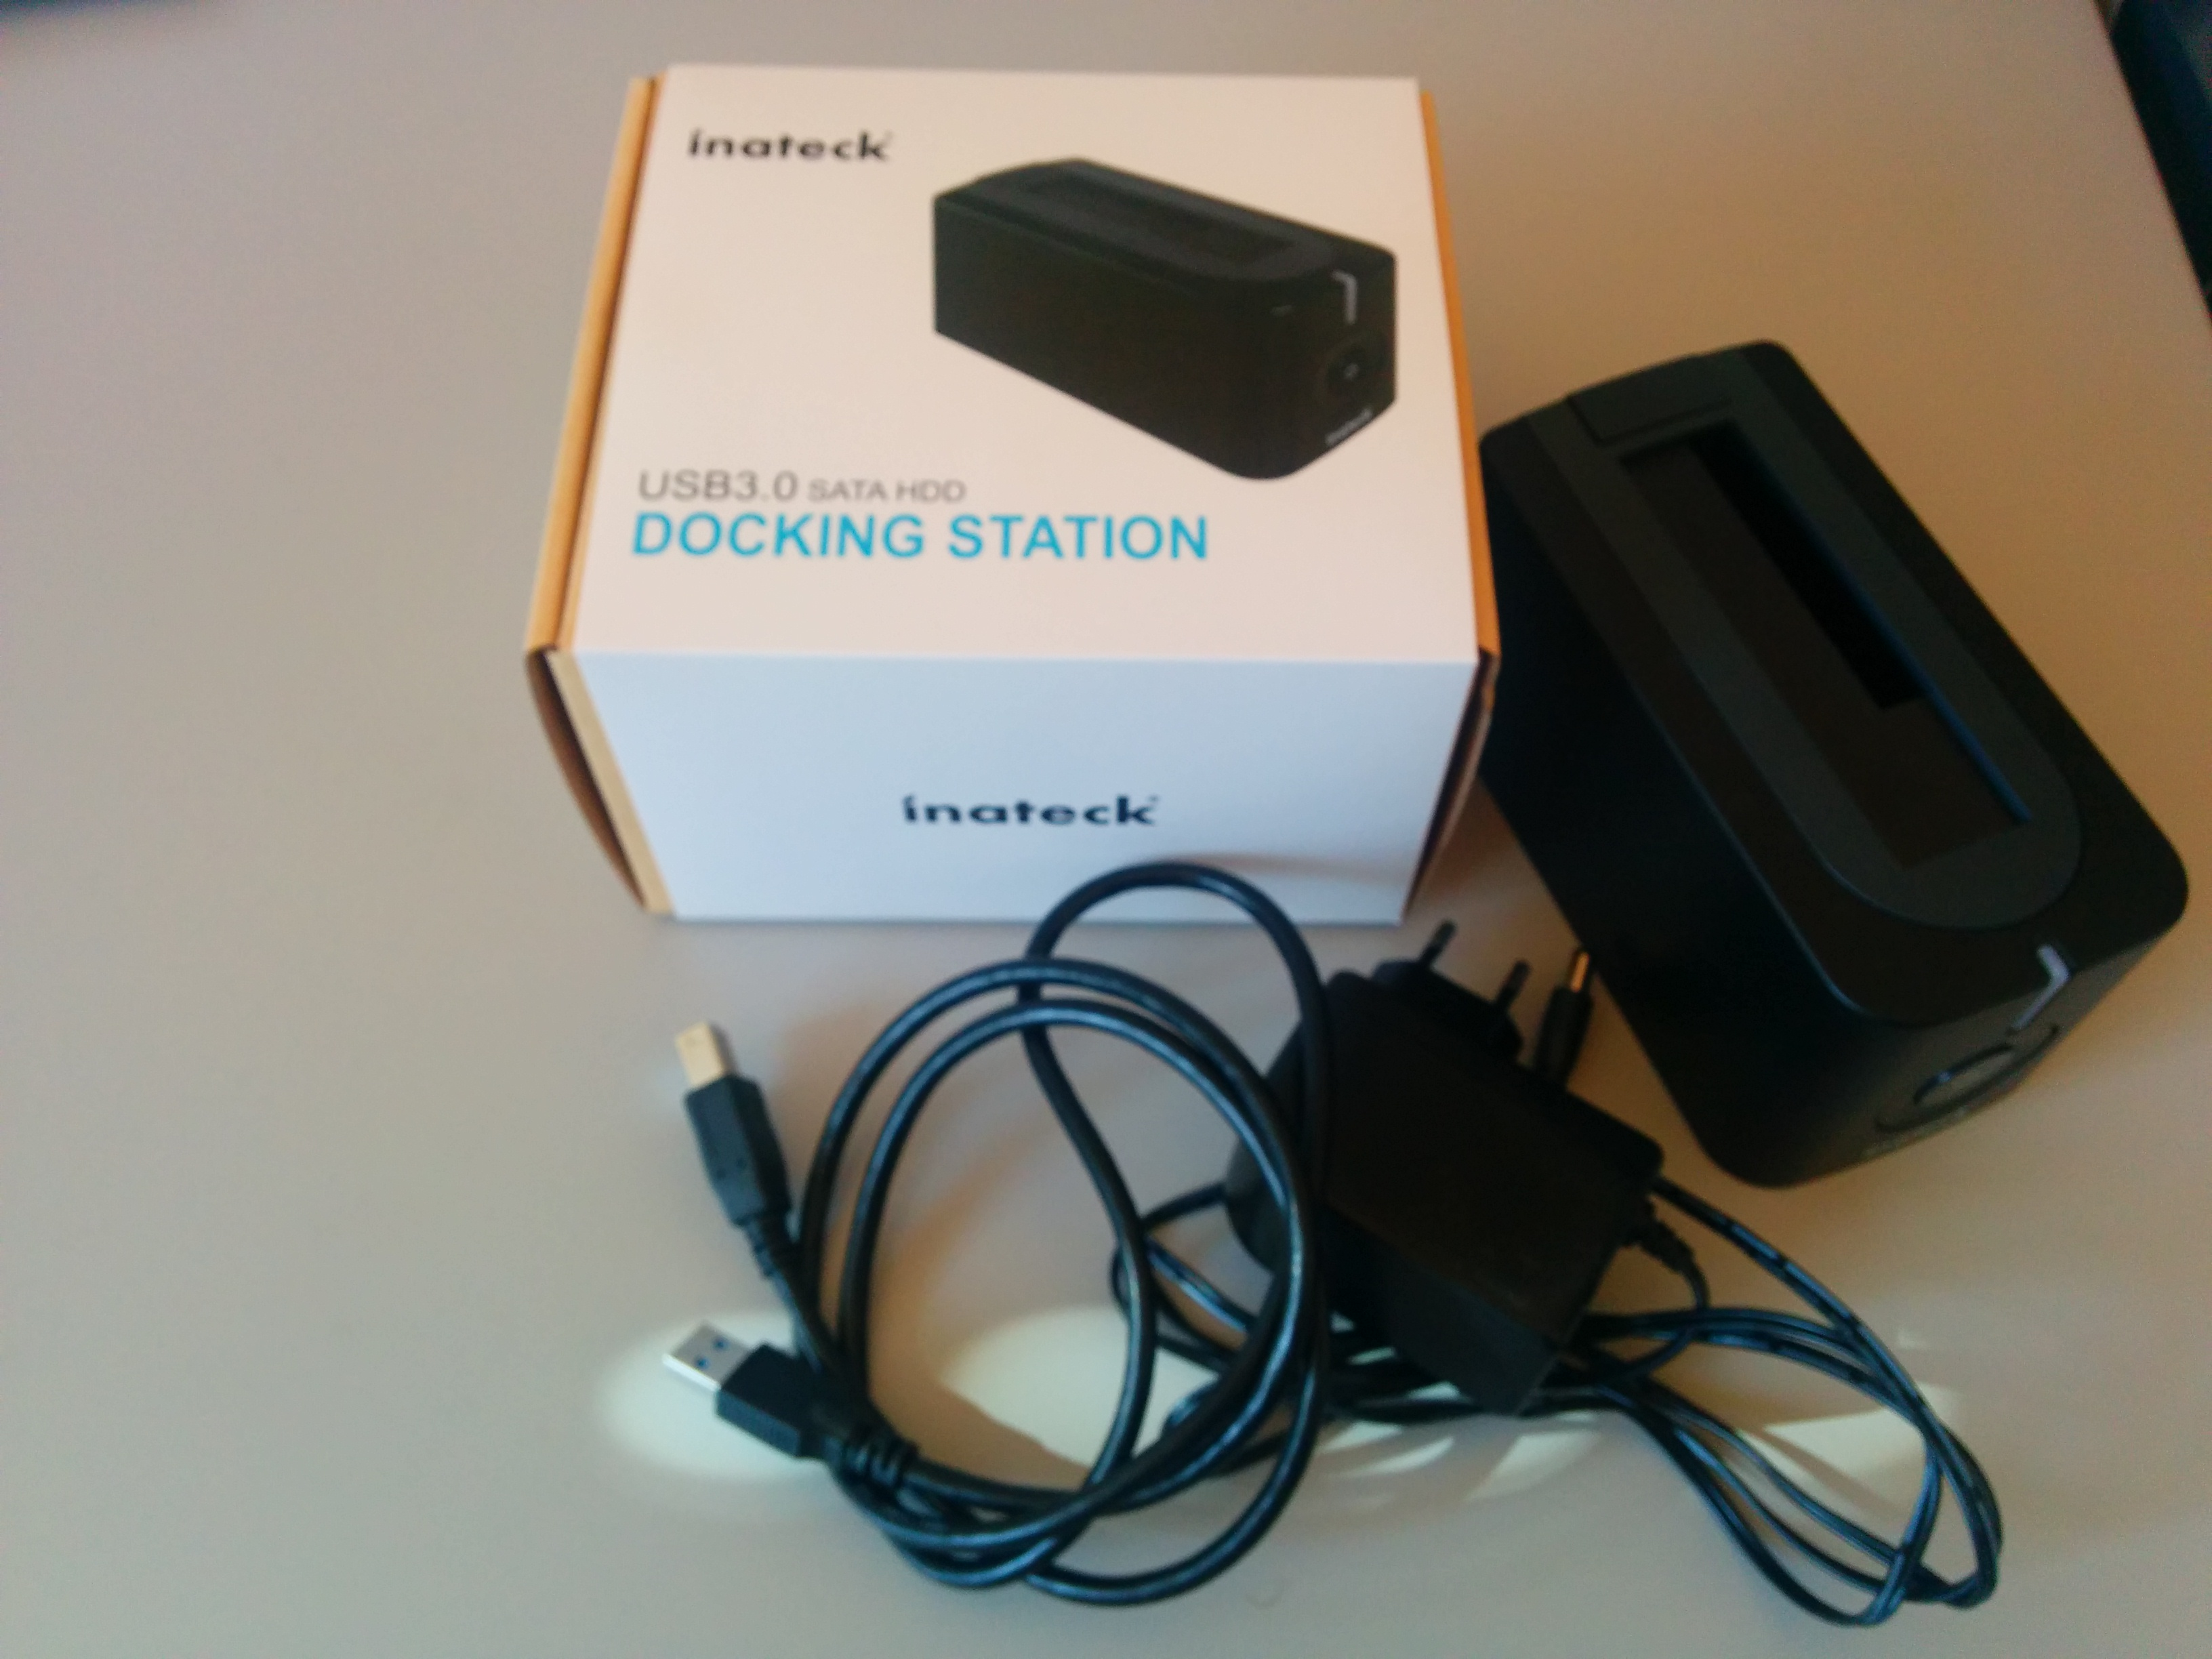
\includegraphics[width=\textwidth]{figures/1_(4).png}
	      \caption{}
		\label{fig_hw_e}
	\end{subfigure}
	\caption{The hardwares}
	\label{fig_hw}
\end{figure}



\subsection{Software}

There are two major aspects which should be taken into account in this work. As it was already mentioned the framework needs both video processing and video editing. Since, there is no open source library to handle both tasks, It is better to stay with C++ or Python. To this end, we checked several libraries and tools listed as follow.

\begin{enumerate}
\item Nuke production:

A software for composing multiple images and effects, motion graphics, not open source, no good documentations. It seems to be for design, film editing, visualization, etc. \url{https://www.thefoundry.co.uk/products/nuke/}

\item MLT framework:

It is an open source tool based on C++ for audio/video editing, media trasncoding, web stream and TV broadcasting. \url{http://www.mltframework.org/}


\item MoviePy:

MoviePy is a Python module for video editing, which can be used for basic operations (like cuts, concatenations, title insertions), video compositing, or to create advanced effects. It can read and write the most common video formats. \url{http://zulko.github.io/moviepy/}

\end{enumerate}

In order to develop new algorithms as convenient as possible, it was decided to take advantages from pre-built libraries and use Python language ( Python 2.7.6 where /usr/bin/python). The required libraries and packages have been listed as below.



\begin{itemize}
	\item ffmpeg
	\item Moviepy
	\item OpenCV-2.4.11	
\end{itemize}

For more details concerning the list of all available python modules, one can use \lq\lq help('modules') \rq\rq in the Python prompt.





\section{Initial Attempts}

\subsection{Camera Setting}

4k Blackmagic camera has different coding formats to store the recorded data and it supports two full HD sizes such as 4k and 2k video . The 4k has 1920x1080 pixels while the size of the 4f video recording is 3840x2160. For each one, there are four different codecs. The codecs are ProRes Proxy, ProRes LT, ProRes 422 and ProRes HQ so that the first one has the lowest quality and the last one takes the highest. Figure \ref{fig_cam} shows the main menu and the sub-menus of the 4k blackmagic camera. This camera has two  disk formats like HFS+ and exFAT (Figure \ref{fig_cam_b}). The former supports Mac OS and the latter works for windows. There in no format for Linux. The most important part of the menu is setting by which one is able to specify various adjustments. The setting part has 4 different sections.  

\begin{enumerate}

	\item Camera (figure \ref{fig_cam_c})

	Here, it is possible to adjust camera Id, date, time, ISO, white balance and shutter angle. In our records, the ISO, white balance and shutter angle have been adjusted into 400, 5200k and 180$^{\circ}$ respectively.

	\item Audio (figure \ref{fig_cam_d})

	The second section is related to audio adjustments and two microphones inputs.

	\item Recording (figure \ref{fig_cam_e})

	The third part supports the recording task and provides different options. In recording format, one can choose either the raw data or one of the 8 codecs. Here, one might determine the fps and time lapse. In our experiments, we use 30 fps.	

	\item Display
	It includes some adjustments corresponding to the screen display of camera like brightness and so on.


\end{enumerate}



\begin{figure}[ht]
	\centering
	\begin{subfigure}[b]{0.30\textwidth}
	       \includegraphics[width=\textwidth]{figures/camera2.png}
	       \caption{The main menu}
		\label{fig_cam_a}
	\end{subfigure} 

	\begin{subfigure}[b]{0.22\textwidth}
	      \includegraphics[width=\textwidth]{figures/camera1.png}
	      \caption{}
		\label{fig_cam_b}
	\end{subfigure}	        
	\begin{subfigure}[b]{0.22\textwidth}
	       \includegraphics[width=\textwidth]{figures/camera3.png}
	       \caption{}
	\label{fig_cam_c}
	\end{subfigure}
	\begin{subfigure}[b]{0.22\textwidth}
	      \includegraphics[width=\textwidth]{figures/camera4.png}
	      \caption{}
		\label{fig_cam_d}
	\end{subfigure}
	\begin{subfigure}[b]{0.22\textwidth}
	      \includegraphics[width=\textwidth]{figures/camera5.png}
	      \caption{}
		\label{fig_cam_e}
	\end{subfigure}
	\caption{The setting menu of Blackmagic camera}
	\label{fig_cam}
\end{figure}


\subsection{ Camera Codec Formats}

The camera has 8 various recording formats as listed in table \ref{table_codecs}. After trying them, we reached the conclusion that base on the fact that the bit-depth of the video for all formats is 10 bits and according to the size, $PSNR$ values and video quality,  the \textbf{4k ProRes Proxy} was chosen to record the videos with 30 frame per second (fps). Moreover, different codings with the appropriate container have been examined as shown in table \ref{table_con}. One can compare the quality of coded videos. The \textbf{.mp4} container and \textbf{x264} coder might be selected as the most promising ones for the final video.

\begin{table}[ht] 
		\centering % used for centering table 
		\caption{The different codecs of 4k Blackmagic camera } 	
		\label{table_codecs} 
		\begin{tabular}{llll} % centered columns (4 columns) 
			 \hline \hline
		Camera codec formats	&  Size (MB/sec) &  Size (GB/90 min) 	&  $PSNR$ \\ 
		\hline
		4k ProRes Proxy 	& 23.1		& 125	& 20 Db	\\
		4k ProRes LT  		& 51.6		& 279	&33 Db	\\
		4k ProRes 422  	& 74.0		& 400	&22 Db	\\
		4k ProRes HQ 		& 108.7		& 587	&99 Db	\\
		2k ProRes Proxy  	& 6.3		& 34		&32 Db	\\
		2k ProRes LT  		& 13.7		& 73		&37 Db	\\
		2k ProRes 422  	& 19.2		& 103	&33 Db	\\
		2k ProRes HQ  	& 28.0		& 151	&99 Db		  
		\end{tabular} 
	\end{table}


\begin{table}[ht] 
		\centering % used for centering table 
		\caption{The different codecs of 4k Blackmagic camera versus different kind of containers and transcoders.
\ding{56} : bad quality , 
\ding{52} : good quality ,
\ding{50} : medium quality} 	
		\label{table_con} 
		\begin{tabular}{llllll} % centered columns (4 columns) 
			 \hline \hline
		Camera codec 	&  .webm   &  .mp4 	&   .mp4  &  .avi  & .agv \\ 
		formats	&  (vpx)  &  (x264)	&    (mpeg4) & (raw video)  & (theora) \\ 
		\hline
		4k ProRes Proxy 	&\ding{50}		& \ding{52}	& \ding{56}		&  \ding{56}	 & \ding{56}	\\
		4k ProRes LT  		&\ding{50}		& \ding{52}	& \ding{56}		&  \ding{56}	 & \ding{56}	\\
		4k ProRes 422  	&\ding{50}		& \ding{52}	& \ding{56}		&  \ding{56}	 & \ding{56}	\\
		4k ProRes HQ 		&\ding{50}		& \ding{52}	& \ding{56}		&  \ding{56}	 & \ding{56}	\\
		2k ProRes Proxy  	&\ding{56}		& \ding{50}	& \ding{56}		&  \ding{56}	 & \ding{56}	\\
		2k ProRes LT  		&\ding{56}		& \ding{52}	& \ding{56}		&  \ding{56}	 & \ding{56}	\\
		2k ProRes 422  	&\ding{50}		& \ding{52}	& \ding{56}		&  \ding{56}	 & \ding{56}	\\
		2k ProRes HQ  	&\ding{50}		& \ding{52}	& \ding{56}		&  \ding{56}	 & \ding{56}		  
		\end{tabular} 
	\end{table}



\begin{figure}[ht]
	\centering
	\begin{subfigure}[b]{0.45\textwidth}
	      \includegraphics[width=\textwidth]{figures/bitrate1.png}
	      \caption{The bitrate of the codecs}
		\label{fig_bit_a}
	\end{subfigure}	        
	\begin{subfigure}[b]{0.45\textwidth}
	       \includegraphics[width=\textwidth]{figures/bitrate2.png}
	       \caption{The size of the codecs}
	\label{fig_bit_b}
	\end{subfigure}

	\begin{subfigure}[b]{0.45\textwidth}
	      \includegraphics[width=\textwidth]{figures/psnr.png}
	      \caption{The PSNR of the codecs}
		\label{fig_bit_c}
	\end{subfigure}
	\caption{Different comparison of the codecs}
	\label{fig_cam}
\end{figure}





\section{Acknowledgments}

I would like to express my very great appreciation to all of team members, Michael Hirsch, Senya Polikovsky, Edgar Klenske, Michael Schober and Parnia Bahar for their patient, valuable and constructive suggestions during this research work.



\end{document}




